\begin{qu}\num
The two circuits are different, but they're made out of identical
batteries and lightbulbs. How do the currents compare?

\vspace{20mm}

\includegraphics{electromagnetism/figs/parallel-not-fixed-current}

\vspace{20mm}

A. $I_2$ and $I_3$ are each about half as big as $I_1$.

B. $I_2$ and $I_3$ are each about the same as $I_1$.

C. $I_2$ and $I_3$ are each about twice as big as $I_1$.

D. There is no way to tell without more data.
\end{qu}
